\documentclass[twocolumn]{article}
\usepackage{amsmath}
\usepackage{amssymb}
\usepackage{graphicx}

\begin{document}

\section*{Numbers}

\begin{itemize}
\item Natural Numbers: $\mathbb{N} = \{1,2,3, \ldots\}$
\item Whole Numbers: $\mathbb{N} \cup \{0\} =\{0,1,2,3, \ldots\}$
\item Integers: $\mathbb{Z} =\{\ldots,-2,-1,0,1,2, \ldots\}$
\item Rational Numbers: $\mathbb{Q} = \left\{\frac{a}{b} \ : \  a, b \in \mathbb{Z} \ , \ b \neq 0 \right\}$. Rational Numbers comprise of fractions (includes all proper and improper fractions and mixed numbers). All terminating decimals (eg, $10.87$) and recurring decimals (eg, $0.3\dot{7}\dot{1} = 0.3717171\ldots$) are rational numbers because these can all be expressed as fractions. All integers are rational numbers.
\item Irrational Numbers: numbers that cannot be expressed in the form $\frac{a}{b}$, where $a$ and $b$ are integers and $b \neq 0$. Eg. $\pi$, $\sqrt{2}$, $\sqrt{5}$, $-4\sqrt{7}$, $e$, $2.75e$, etc. Irrational numbers are non-recurring decimals. Any non-zero rational number multiplied to an irrational number results in an irrational number. For example, $-\frac{3}{4}\pi$ is irrational.
\item Perfect Squares: $\{1,4,9,16,25, \ldots\}$
\item Perfect Cubes: $\{1,8,27,64, \ldots\}$
\item Prime Numbers: Positive integers at least 2 whose only positive divisors are 1 and itself. $\{2,3,5,7,11,13,17,19,23, \ldots\}$
\item Composite Numbers: Positive integers $\geq 4$ that are not prime, in other words, having positive divisors apart from 1 and itself.
\end{itemize}

\section*{Equality and Inequality Symbols}

\begin{tabular}{|c|l|l|}
	\hline Symbol & \multicolumn{1}{|c|}{ Meaning } & \multicolumn{1}{|c|}{ Example } \\
	\hline$=$ & is equal to & $0.1=\frac{1}{10}$ \\
	\hline$\neq$ & is not equal to & $0.11 \neq \frac{1}{10}$ \\
	\hline$>$ & is greater than & $0.1>0.01$ \\
	\hline$\geqslant$ & is greater than or equal to & $a \geqslant 5$ \\
	\hline$<$ & is less than & $0.05<5$ \\
	\hline$\leqslant$ & is less than or equal to & $b \leqslant 5$ \\
	\hline
\end{tabular}

\section*{Prime Factorization, HCF, LCM} 

\begin{itemize}
\item Example of prime factorization:

\begin{tabular}{r|c}
	2 & 4356 \\
	\cline { 2 - 2 } 2 & 2178 \\
	\cline { 2 - 2 } 3 & 1089 \\
	\cline { 2 - 2 } 3 & 363 \\
	\cline { 2 - 2 } 11 & 121 \\
	\cline { 2 - 2 } & 11 \\
	\hline 
\end{tabular}

Hence $4356=2^2 \times 3^2 \times 11^2$ (in index notation).

\item Example of HCF and LCM using prime factorization:

$
\begin{aligned}
	& 4800=2^6 \times 3 \times 5^2 \\
	& 5544=2^3 \times 3^2 \times 7 \times 11
\end{aligned}
$

$\mathrm{HCF}=2^3 \times 3$

[take common prime factors and lowest power of each]

$\mathrm{LCM}=2^6 \times 3^2 \times 5^2 \times 7 \times 11$

[take all prime factors and highest power of each]

\item Examples of square roots and cube roots using prime factorization:

$\begin{aligned} 54756 & =2^2 \times 3^4 \times 13^2 \\ \sqrt{54756} & =2 \times 3^2 \times 13 = 234\end{aligned}$

$\begin{aligned} 1728 & =2^6 \times 3^3 \\ \sqrt[3]{1728} & =2^2 \times 3 = 12\end{aligned}$
\end{itemize}

\section*{Approximation}

\subsection*{Significant Figures}

\noindent
Rules of identifying number of significant digits:

\begin{enumerate} 
\item All non-zero digits are significant.
\item Zeros between non-zero digits are significant. 

Eg. 302 (3 sf)

Eg. 10.2301 (6 sf)

\item In a whole number, zeros after the last nonzero digit may or may not be significant. It depends on the estimation being made.

Eg.

$
\begin{aligned}
	& 7436000=7000000 \ (1 \ \mathrm{sf}) \\
	& 7436000=7400000 \ (2 \ \mathrm{sf}) \\
	& 7436000=7440000 \ (3 \ \mathrm{sf}) \\
	& 7436000=7436000 \ (4 \ \mathrm{sf}) \\
	& 7436000=7436000 \ (5 \ \mathrm{sf}) \\
	& 7436000=7436000 \ (6 \ \mathrm{sf}) \\
\end{aligned}
$

\item In a decimal number, zeros before the $1^{\text{st}}$ non-zero digit are not significant.

Eg. $0.004 \ (1 \ \mathrm{sf})$

Eg. $0.07008 \ (4 \ \mathrm{sf})$

\item In a decimal number, zeros after the last non-zero digit are significant.

Eg. $6.40 \ (3 \ \mathrm{sf})$

Eg. $12.000 \ (5 \ \mathrm{sf})$

Eg. $20300.000 \ (8 \ \mathrm{sf})$

Eg. $0.0700800 \ (6 \ \mathrm{sf})$
\end{enumerate} 

\subsection*{Decimal Place Rounding}

\noindent 
Examples:

\noindent
$
\begin{aligned}
	& 0.7374=0.74 \ (2 \ \mathrm{dp}) \\
	& 58.301=58.30 \ (2 \ \mathrm{dp}) \\
	& 207.6296=207.630 \ (3 \ \mathrm{dp}) \\
	& 207.6296=207.63 \ (2 \ \mathrm{dp}) \\
    & 207.977=208.0 \ (1 \ \mathrm{dp}) \\
    & 207.977=207.98 \ (2 \ \mathrm{dp}) \\
    & 18.997=19.00 \ (2 \ \mathrm{dp})
\end{aligned}
$

\section*{Standard Form}

\noindent
$\pm A \times 10^n$, where $1 \leq A < 10$ and $n$ is an integer.

\bigskip 

\noindent
Examples:

\noindent
$
\begin{aligned}
	& 1350000=1.35 \times 10^6 \\
	& 0.000375=3.75 \times 10^{-4}
\end{aligned}
$

\section*{Common Prefixes}

\begin{tabular}{|l|l|l|l|}
	\hline $10^{12}$ & trillion & tera & $\mathrm{T}$ \\
	\hline $10^9$ & billion & giga & $\mathrm{G}$ \\
	\hline $10^6$ & million & mega & $\mathrm{M}$ \\
	\hline $10^3$ & thousand & kilo & $\mathrm{k}$ \\
	\hline $10^{-3}$ & thousandth & milli & $\mathrm{m}$ \\
	\hline $10^{-6}$ & millionth & micro & $\mu$ \\
	\hline $10^{-9}$ & billionth & nano & $\mathrm{n}$ \\
	\hline $10^{-12}$ & trillionth & pico & $\mathrm{p}$ \\
	\hline
\end{tabular}

\section*{Indices}

\noindent 
Rules of Indices:

\bigskip 

\noindent 
Assume that $a,b,m,n$ are non-zero.

\noindent 
$\begin{gathered} a^0=1 \\ a^m \times a^n=a^{m+n} \\ a^m \div a^n=a^{m-n} \\ (a b)^n=a^n b^n \\ \left(\frac{a}{b}\right)^n=\frac{a^n}{b^n} \\ \left(a^n\right)^m=a^{n m} \\ a^{-n}=\frac{1}{a^n} \\ \left(\frac{a}{b}\right)^{-n}=\left(\frac{b}{a}\right)^n=\frac{b^n}{a^n} \\  a^{\frac{1}{n}}=\sqrt[n]{a} \\ a^{\frac{m}{n}}=\sqrt[n]{a^m}=(\sqrt[n]{a})^m\end{gathered}$

\noindent
Caution:

\noindent
1. For indices (powers) that are not integers, the above rules of indices hold only for $a,b > 0$.

\noindent
2. Likewise, if some of the indices are negative or there is division by either $a$ or $b$, then the above rules hold only for $a,b > 0$.

\noindent
3. $\sqrt{(-8)^2} = \sqrt{64} = 8$, NOT $-8$.

\noindent
4. $\sqrt[3]{-27} = -3$.

\bigskip 

\noindent 
Equalities of Indices:

\noindent 
1. If $a^m=a^{\prime \prime}$, then $m=n$.

\noindent 
2. If $a^m=b^m$, then $a=b$.

\section*{Percentage, Ratio, Rate}

\begin{itemize}  

\item To express a percentage as a fraction or decimal, divide by $100$:

$
x \%=\frac{x}{100}
$

Eg, $23.5 \% = \frac{23.5}{100} = \frac{235}{1000} = \frac{47}{200}$

Eg, $401 \% = \frac{401}{100} = 4.01$

\item To express any number as a percentage, multiply it by $100 \%$.

Eg, $0.165 = 0.165 \times 100 \% = 16.5 \%$.

\item Expressing a quantity $A$ as a percentage of a quantity $B$:

$
\frac{A}{B} \times 100 \%
$

Eg, Express $63.7$ as a percentage of $98$. 

Answer: $\frac{63.7}{98} \times 100\% = 65 \%$

In words, we say that $63.7$ is $65 \%$ of $98$. 

\item Increase or decrease a quantity by a given percentage:

Eg, Increase $45$ by $2.4 \%$:

Answer: $45 \times \left(1+\frac{2.4}{100}\right) = 45 \times 1.024 = 46.08$  

Eg, Decrease $45$ by $90 \%$:

Answer: $45 \times \left(1-\frac{90}{100}\right) = 45 \times 0.1 = 4.5$

\item Percentage Increase and Percentage Decrease:

When a quantity increases, the percentage increase is

$\frac{\text{final value} \ - \ \text{initial value}}{\text{initial value}} \times 100\%$

When a quantity dereases, the percentage decrease is

$\frac{\text{initial (bigger) value} \ - \ \text{final (smaller) value}}{\text{initial value}} \times 100\%$

Percentage increase will always be $> 0$ if the quantity has increased.

Percentage decrease will always be $> 0$ if the quantity has decreased.

Percentage change is

$\frac{\text{final value} \ - \ \text{initial value}}{\text{initial value}} \times 100\%$

regardless of whether the quantity has increased or decreased. Percentage change can be either positive or negative depending on whether the quantity has increased or decreased.

\item When writing ratios such as $a:b$, $a,b$ are positive integers. Always reduce ratios to the simplest form, eg, $10:6$ is to be reduced to $5:3$. The ratio $a:b$ expressed in fraction form is $\frac{a}{b}$.

Eg, If 7 times of $x$ is equal to 5 times of $y$, then $x:y = 5:7$ (note the switching of the order)

\item We can use ratios to increase and decrease quantities.
For example, if we increase a quantity $x$ in the ratio $6: 5$, the new quantity is $\frac{6}{5} x$; if we decrease a quantity $x$ in the ratio $5: 6$, the new quantity is $\frac{5}{6} x$.

\item Various units of measurement:

Mass:

$1 \ \text{kg} = 1000 \ \text{g}$ 

$1 \ \text{g} = 1000 \ \text{mg}$

Length:

$1 \ \text{km} = 1000 \ \text{m}$

$1 \ \text{m} = 100 \ \text{cm}$

$1 \ \text{cm} = 10 \ \text{mm}$

Area:

$1 \ \text{km}^2 = 10^6 \ \text{m}^2$

$1 \ \text{m}^2 = 10000 \ \text{cm}^2$

Volume:

$1 \ \text{\it l} = 1000 \ \text{ml}$ 

$1 \ \text{cm}^3 = 1 \ \text{ml}$ 

$1 \ \text{m}^3 = 10^6 \ \text{cm}^3 = 1000 \ \text{\it l}$ 

Time:

$1 \ \text{hr} = 60 \ \text{min}$ 

$1 \ \text{min} = 60 \ \text{sec}$ 

\item Distance = Speed $\times$ Time

\item Average speed = (Total Distance) $/$ (Total Time Taken)

\item Conversion of units for speed:

$26 \text{km}/\text{h} = 26000 \text{m}/\text{h} = \frac{26000}{3600}  \text{m}/\text{s} = \frac{65}{9} \text{m}/\text{s} $

$35 \text{m}/\text{s} = 0.035 \text{km}/\text{s} = (0.035 \times 3600) \text{km}/\text{h} = 126 \text{km}/\text{h}$

\item Density = Mass $/$ Volume.

Units are usually $\text{g}/\text{cm}^3$ or $\text{kg}/\text{m}^3$.

$1 \text{g}/\text{cm}^3 = 1000 \text{kg}/\text{m}^3$.

Eg, $0.235 \text{g}/\text{cm}^3 = 235 \text{kg}/\text{m}^3$.

\end{itemize}  

\section*{Direct and Inverse Proportion}

\noindent 
If $y$ is directly proportional to $x$, then $y=k x$, where $k$ is a constant and $k \neq 0$. The ratios $\frac{x}{y}$ and $\frac{y}{x}$ are constant. Furthermore, the graph on $y$ against $x$ (or of $x$ against $y$) is a straight line through the origin.

\noindent
Graph showing that $y$ is directly proportional to  $x$:

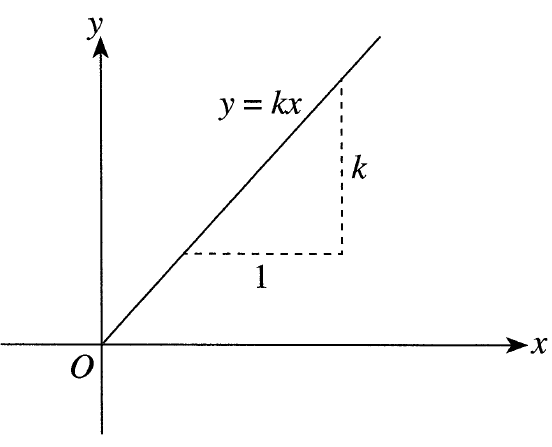
\includegraphics[width=0.3\textwidth]{01.png}

\bigskip 

\noindent 
If $y$ is inversely proportional to $x$, then $y=\frac{k}{x}$, where $k$ is a constant and $k \neq 0$. The product $xy$ is constant. 

\noindent
Graph showing that $y$ is inversely proportional to  $x$:

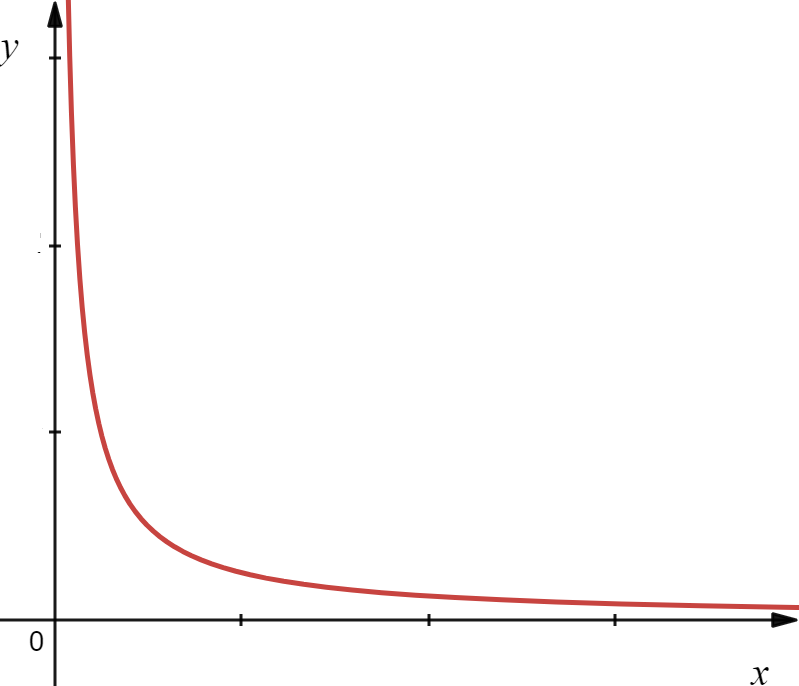
\includegraphics[width=0.3\textwidth]{02.png}

\section*{Map Scales}

\begin{itemize}  
	
	\item Linear scale:
	
	$1: n$ means $1$ unit length on map represents $n$ units length on ground.
	
	Eg. $1 : 5000$ means
	
	$1 \mathrm{~cm}$ represents $5000 \mathrm{~cm}$
	
	which implies $1 \mathrm{~cm}$ represents $50 \mathrm{~m}$
	
	which implies $1 \mathrm{~cm}$ represents $0.05 \mathrm{~km}$
	
	\item Representative Fraction (RF):
	
	If the linear scale is $1:n$, the RF is expressed as $\frac{1}{n}$.
	
	Eg, if 3 cm represents 6 m, then RF is $\frac{1}{200}$.
	
	\item Area Scale:
	
	If linear scale is $1:20000$, then it means 
	
	$1 \mathrm{~cm}$ represents $20000 \mathrm{~cm}$
	
	which implies  $1 \mathrm{~cm}$ represents $0.2 \mathrm{~km}$
	
	which implies $1^2 \mathrm{~cm}^2$ represents $(0.2)^2 \mathrm{~km}^2$
	
	which implies $1 \mathrm{~cm}^2$ represents $0.04 \mathrm{~km}^2$

\end{itemize} 

\section*{Number Patterns}

\noindent
Common number patterns:

\begin{itemize}  
	
\item Constant difference

Eg, $-5, -2, 1, 4, 7, 10, \ldots$

The $n^{\text{th}}$ term, denoted $T_n$, is given by

$T_n = a + d(n-1)$

where $a$ is the first term and $d$ is the common difference.

For the sequence $-5, -2, 1, 4, 7, 10, \ldots$, 

$T_n = -5 + (n-1)(3) = 3n - 8$.

Alternatively,

$T_n = b + dn$

where $b$ is the term that would have come before the first term (ie, the ``zeroth'' term).

\item Constant multiple (or common ratio)

Eg, $3, 15, 75, 375, \ldots$

$T_n = a \times r^{n-1}$

where $a$ is the first term, $r$ is the common ratio, that is, $r$ is the number that when multiplied a term gives the next term.

For the sequence $3, 15, 75, 375, \ldots$

$T_n = 3 \times 5^{n-1}$.

\item Perfect squares and perfect cubes

$1, 4, 9, 16, 25, \ldots \ : \ T_n = n^2$

$1, 8, 27, 64, 125, \ldots \ : \ T_n = n^3$

$2, 8, 18, 32, 50, \ldots \ : \ T_n = 2n^2$

$3, 10, 29, 66, 127, \ldots \ : \ T_n = n^3+2$

\item Fibonacci Sequences

Each term is the sum of the previous two terms:

$1, 1, 2, 3, 5, 8, 13, 21, 34, 55, \ldots$

$-2, 3, 1, 4, 5, 9, 14, 23, 37, \ldots$
	
\end{itemize}  	

\section*{Simultaneous Linear Equations}

Method 1: Elimination

$
\begin{gathered}
	5 x-2 y=21 \ \ \ \text{---(1)}\\
	2 x-y=8 \ \ \ \text{---(2)}
\end{gathered}
$

$\text{(1)} \times 2: 10 x-4 y=42  \ \ \ \text{---(3)}$

$\text{(2)}\times 5: 10 x-5 y=40  \ \ \ \text{---(4)}$

$\text{(3) - (4)}: \quad y=2$

Sub into (1): $5 x-2(2)=21$

$5 x-4 =21 \ \Rightarrow \ 5 x =25 \ \Rightarrow \	x =5$

\bigskip 

\noindent 
Method 2: Substitution

$
\begin{gathered}
	5 x-2 y=21 \ \ \ \text{---(1)} \\
	2 x-y=8 \ \ \ \text{---(2)}
\end{gathered}
$

From (2):

$
y=2 x-8  \ \ \ \text{---(3)}
$

Sub (3) into (1): $5 x-2(2 x-8)=21$

$
\begin{aligned}
	5 x-4 x+16 & =21 \ \Rightarrow \ x-16 & =21 \\
	x & =5
\end{aligned}
$

Sub into (2):

$	2(5)-y=8 \ \Rightarrow \ 10-y=8 \ \ \Rightarrow  \	y=2 $

\section*{Inequalities}

\noindent 
Inequality sign is reversed when both sides are multiplied or divided by a negative number.

\bigskip 

\noindent 
Eg. $-3x + 4  \geq 12$

$-3x \geq 12-4$

$-3x \geq 8$

$x \leq - \frac{8}{3}$

\bigskip 

\noindent 
Eg. $3(x-1)<4 x+1 \leq 7+2 x$

\bigskip 
\begin{tabular}{c|c} 
	$
	\begin{aligned}
		& 3(x-1)<4 x+1 \\
		& 3 x-3<4 x+1 \\
		& 3 x-4 x<1+3 \\
		& -x<4 \\
		& x>-4
	\end{aligned}
	$
	& 
	$
	\begin{aligned}
		& 4 x+1 \leq 7+2 x \\
		& 4 x-2 x \leq 7-1 \\
		& 2 x \leq 6 \\
		& x \leq 3 \\
		& ~
	\end{aligned}
	$
\end{tabular} 

\bigskip 

\noindent 
Ans: $-4 < x \leq 3$

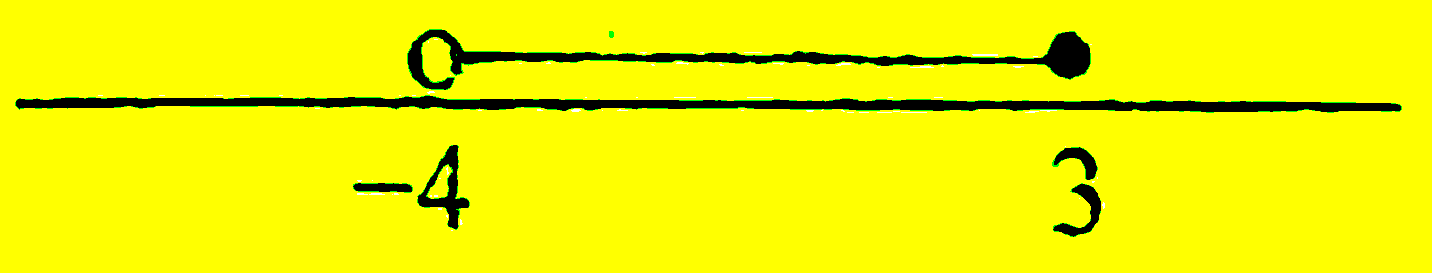
\includegraphics[width=0.3\textwidth]{03.png}

\bigskip 

\noindent 
Eg. $5 x+4 \leq 3 x<6-3 x$

\bigskip 
\begin{tabular}{c|c} 
	$
	\begin{aligned}
		5 x+4 & \leq 3 x \\
		2 x & \leq-4\\
		x & \leq-2
	\end{aligned}
	$
	& 
	$
	\begin{aligned}
		3 x & <6-3 x \\
		6 x & <6 \\
		x & <1
	\end{aligned}
	$
\end{tabular} 

\bigskip 

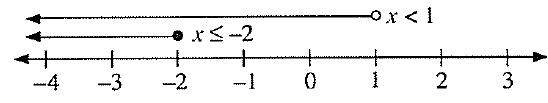
\includegraphics[width=0.4\textwidth]{04.png}

\noindent 
Ans: $x \leq -2$.

\section*{Expansion}

\noindent
Eg.

\noindent
$
\begin{aligned}
	& 2 p-3(p+1) \\
	= & 2 p-3 p-3 \\
	= & -p-3
\end{aligned}
$

\noindent
Eg.

\noindent
$
\begin{aligned}
	& 5 x-(x+1)(2 x-3) \\
	= & 5 x-\left(2 x^2-3 x+2 x-3\right) \\
	= & 5 x-2 x^2+3 x-2 x+3 \\
	= & -2 x^2+6 x+3
\end{aligned}
$

\section*{Factorization and Identities}

\noindent
Factorization of Quadratic Expressions:

\noindent
$
5 x^2+9 x-2
$

\begin{tabular}{c|c|c|}
	$\times$ & \multicolumn{1}{|c}{$5 x$} & $-1$ \\
	\hline$x$ & $5 x^2$ & $-x$ \\
	\cline { 2 - 3 } $2$ & $10 x$ & $-2$ \\
	\hline 
\end{tabular}

\noindent 
$
\therefore \ \ 5 x^2+9 x-2=(5 x-1)(x+2)
$

\bigskip 

\noindent 
Identities:

\bigskip 

\noindent 
1. $(a+b)^2=a^2+2 a b+b^2$

\noindent 
2. $(a-b)^2=a^2-2 a b+b^2$

\noindent 
3. $(a+b)(a-b)=a^2-b^2$

\bigskip 

\noindent 
Common Factorisation Techniques:

\begin{itemize} 
\item Common Factors

Eg. $6 a^3 b-2 a^2 b=2 a^2 b(3 a-1)$

\item Grouping

Eg.

$
\begin{aligned}
	& 6 p^2-3 p q-10 a p+5 a q \\
	& =3 p(2 p-q)-5 a(2 p-q) \\
	& =(3 p-5 a)(2 p-q)
\end{aligned}
$

\item Using Difference of Two Squares

$
\begin{aligned}
	& \text { Eg. } 9 a^2-1 \\
	& =(3a)^2 - (1)^2 \\
	& =(3 a+1)(3 a-1)
\end{aligned}
$

\noindent 
$
\begin{aligned}
	& \text { Eg. } 16 a^4-81 \\
	& =(4a^2+9)(4a^2-9) \\
	& =(4a^2+9)(2a+3)(2a-3)
\end{aligned}
$

\item Combination of methods:

Eg. $3 x^3-12 x y^2$
$=3 x\left(x^2-4 y^2\right)$ common factor
$=3 x(x+2 y)(x-2 y)$ then diff. of 2 squares

Always try common factor first

Eg.

$
\begin{aligned}
	& 4 - p^2 + 6pq - 9q^2  \\
	& =4 - (p^2 - 6pq + 9q^2) \\
	& =(2)^2 - (p-3q)^2 \\
	& =(2+(p-3q))(2-(p-3q)) \\
	& =(2+p-3q)(2-p+3q)
\end{aligned}
$

\end{itemize} 

\section*{Algebraic Fractions}

\noindent 
Eg.

\noindent 
$
\begin{aligned}
	& \frac{x+2}{3}-\frac{x-5}{2}=\frac{2(x+2)}{6}-\frac{3(x-5)}{6} \\	
	& =\frac{2(x+2)-3(x-5)}{6} \\
	& =\frac{2 x+4-3 x+15}{6} \\
	& =\frac{19-x}{6}
\end{aligned}
$

\bigskip 

\noindent 
Eg.

\noindent 
$
\begin{aligned}
	& \frac{5}{x+1}-\frac{2}{x-3} \\
	& =\frac{5(x-3)}{(x+1)(x-3)}-\frac{2(x+1)}{(x-3)(x+1)} \\
	& =\frac{5(x-3)-2(x+1)}{(x+1)(x-3)} \\
	& =\frac{5 x-15-2 x-2}{(x+1)(x-3)} \\
	& =\frac{3 x-17}{(x+2)(x-5)}
\end{aligned}
$

\bigskip 

\noindent 
Eg.

\noindent 
$
\begin{aligned}
	& \frac{5}{3 x}+\frac{2}{x} \\
	& = \frac{5}{3 x}+\frac{6}{3x} \\
	& =\frac{5+6}{3 x} \\
	& =\frac{11}{3 x}
\end{aligned}
$

\bigskip 

\noindent 
Eg. 

\noindent 
$
\begin{aligned}
	& \frac{3}{(x+2)^2}-\frac{4}{x+2} \\
	& =\frac{3}{(x+2)^2}-\frac{4(x+2)}{(x+2)^2} \\	
	& =\frac{3-4(x+2)}{(x+2)^2} \\
	& =\frac{3-4 x-8}{(x+2)^2} \\
	& =\frac{-4 x-5}{(x+2)^2}
\end{aligned}
$

\bigskip 

\noindent 
Eg. 

\noindent 
$
\begin{aligned}
	& \frac{7}{x^2-9}-\frac{1}{x-3} \\
	& =\frac{7}{(x+3)(x-3)}-\frac{1}{x-3} \\
	& =\frac{7}{(x+3)(x-3)}-\frac{x-3}{(x-3)^2} \\	
	& =\frac{7-(x+3)}{(x+3)(x-3)} \\
	& =\frac{7-x-3}{(x+3)(x-3)} \\
	& =\frac{4-x}{(x+3)(x-3)}
\end{aligned}
$

\bigskip 

\noindent 
Eg. 

\noindent 
$\begin{aligned} & \frac{3 x+2}{x^2-4}+\frac{1}{x+2}-\frac{2}{x-2} \\ &= \frac{3 x+2}{(x+2)(x-2)}+\frac{1}{x+2}-\frac{2}{x-2} \\ &= \frac{3 x+2+(x-2)-2(x+2)}{(x+2)(x-2)} \\ &= \frac{3 x+2+x-2-2 x-4}{(x+2)(x-2)} \\ &= \frac{2 x-4}{(x+2)(x-2)} \\ &= \frac{2(x-2)}{(x+2)(x-2)} \\ &= \frac{2}{x+2}\end{aligned}$

\bigskip 

\noindent 
Eg. 

\noindent 
$
\begin{aligned}
	& \frac{9}{x-5}+\frac{3}{5-x} \\
	& =\frac{9}{x-5}-\frac{3}{x-5} \\
	& =\frac{9-3}{x-5} \\
	& =\frac{6}{x-5}
\end{aligned}
$

\bigskip 

\bigskip 

\bigskip 

\bigskip 

\bigskip 

\bigskip 

\bigskip 

\bigskip 

\noindent 
Eg. 

\noindent 
$\begin{aligned} & \frac{2 x}{3 y-8 x}+\frac{11 x}{80 x-30 y} \\ = & \frac{2 x}{3 y-8 x}+\frac{11 x}{-10(3 y-8 x)} \\ = & \frac{2 x}{3 y-8 x}-\frac{11 x}{10(3 y-8 x)} \\ = & \frac{20 x-11 x}{10(3 y-8 x)} \\ = & \frac{9 x}{10(3 y-8 x)}\end{aligned}$

\bigskip 

\noindent 
Eg. 

\noindent 
$\begin{aligned} & \frac{4}{x^2-4}+\frac{1}{2-x} \\ = & \frac{4}{(x+2)(x-2)}-\frac{1}{x-2} \\ = & \frac{4-(x+2)}{(x+2)(x-2)} \\ = & \frac{4-x-2}{(x+2)(x-2)} \\ = & \frac{2-x}{(x+2)(x-2)} \\ = & \frac{-x-2)}{(x+2)(x-2)} \\ = & -\frac{1}{x+2}\end{aligned}$

\bigskip 

\noindent 
Eg. 

\noindent 
$\begin{aligned} & \frac{6 p^3}{7 q} \div \frac{2 p}{21 q^2} \\ = & \frac{6 p^3}{7 q} \times \frac{21 q^2}{2 p} \ \ [\text { do cancelling }] \\ = & 9 p^2 q\end{aligned}$

\bigskip 

\noindent 
Eg. 

\noindent 
$\begin{aligned} \frac{4 p q^2+4 p q r}{9 p q r^2+9 p q^2 r} & =\frac{4 p q(q+r)}{9 p q r(r+q)} \\ & =\frac{4}{9 r}\end{aligned}$

\bigskip 

\bigskip 

\bigskip 

\bigskip 

\bigskip 

\bigskip 

\noindent 
Eg. 

\noindent 
$\begin{aligned} \frac{5 k^2-17 k-12}{5 k^2-10 k-40} & =\frac{(5 k+3)(k-4)}{5\left(k^2-2 k-8\right)} \\ & =\frac{(5 k+3)(k-4)}{5(k-4)(k+2)} \\ & =\frac{5 k+3}{5(k+2)}\end{aligned}$

\bigskip 

\noindent 
Eg. 

\noindent 
$\begin{aligned} & \frac{x y-z^2-x z+y z}{y^2-2 y z+z^2} \div \frac{11}{2 x z+x^2+z^2} \\ & =\frac{x y-x z+y z-z^2}{y^2-2 y z+z^2} \times \frac{2 x z+x^2+z^2}{11} \\ & =\frac{x(y-z)+z(y-z)}{(y-z)^2} \times \frac{(x+z)^2}{11} \\ & =\frac{(x+z)(y-z)}{(y-z)^2} \times \frac{(x+z)^2}{11} \\ & =\frac{(x+z)^3}{11(y-z)}\end{aligned}$

\bigskip 

\noindent 
Eg. 

\noindent 
$\begin{aligned} & \frac{1}{x}+1 \\ & =\left(\frac{1}{x}+1\right) \div(x+1) \\ & =\frac{1+x}{x} \times \frac{1}{x+1} \\ & =\frac{1}{x}\end{aligned}$

\bigskip 

\noindent 
Eg. 

\noindent 
$\begin{aligned} & \frac{1-\frac{1}{x}}{1-\frac{1}{x^2}} \\ & =\left(1-\frac{1}{x}\right) \div\left(1-\frac{1}{x^2}\right) \\ & =\left(\frac{x-1}{x}\right) \div\left(\frac{x^2-1}{x^2}\right) \\ & =\frac{x-1}{x} \times \frac{x^2}{x^2-1^2} \\ & =\frac{x-1}{x} \times \frac{x^2}{(x+1)(x-1)} \\ & =\frac{x}{x+1}\end{aligned}$

\section*{Making Subject of Formula}

\bigskip 

\noindent 
Eg: Make $a$ the subject

\noindent 
$\begin{aligned} y & = m(x-a)+b \\ y-b & =m(x-a) \\ m(x-a) & =y-b \\ x-a & =\frac{y-b}{m} \\ a & =x-\frac{y-b}{m}\end{aligned}$

\bigskip 

\noindent 
Eg: Make $x$ the subject

\noindent 
$\begin{aligned} a x-b y & =3-2 x \\ a x+2 x & =3+b y \\ x(a+2) & =b y+3 \\ x & =\frac{b y+3}{a+2}\end{aligned}$

\bigskip 

\noindent 
Eg: Make $d$ the subject

\noindent 
$\begin{aligned} T & =0.25 \pi d^2 \\ \pi d^2 & =4 T \\ d^2 & =\frac{4 T}{\pi} \\ d & = \pm \sqrt{\frac{4 T}{\pi}}\end{aligned}$

\noindent
Note the $\pm$ when taking square-roots in this type of question.

\bigskip 

\noindent 
Eg: Make $c$ the subject

\noindent 
$\begin{aligned} d & =\frac{8-c}{c+7} \\ d(c+7) & =8-c \\ c d+7 d & =8-c \\ c d+c & =8-7 d \\ c(d+1) & =8-7 d \\ c & =\frac{8-7 d}{d+1}\end{aligned}$

\bigskip 

\bigskip 

\bigskip 

\bigskip 

\bigskip 

\bigskip 

\bigskip 

\bigskip 

\bigskip 

\noindent 
Eg: Make $q$ the subject

\noindent 
$\begin{aligned} 5 a & =\sqrt{\frac{b^2}{q}-\frac{3 c}{4}} \\ 25 a^2 & =\frac{b^2}{q}-\frac{3 c}{4} \\ \frac{b^2}{q} & =25 a^2+\frac{3 c}{4} \\ \frac{b^2}{q} & =\frac{100 a^2+3 c}{4} \\ \frac{q}{b^2} & =\frac{4}{100 a^2+3 c} \\ q & =\frac{4 b^2}{100 a^2+3 c}\end{aligned}$

\bigskip 

\noindent 
Eg: Make $y$ the subject

\noindent 
$\begin{aligned} \frac{x\left(y z-w^2\right)}{2}-\frac{y}{3} & =6 y \\ 3 x\left(y z-w^2\right)-2 y & =36 y \\ 3 x y z-3 w^2 x-2 y & =36 y \\ 3 x y z-38 y & =3 w^2 x \\ y(3 x z-38) & =3 w^2 x \\ y & =\frac{3 w^2 x}{3 x z-38}\end{aligned}$

\bigskip 

\noindent 
Eg: Make $x$ the subject

\noindent 
$\begin{aligned} p \sqrt{x}+q & =r+s \sqrt{x} \\ p \sqrt{x}-s \sqrt{x} & =r-q \\ \sqrt{x}(p-s) & =r-q \\ \sqrt{x} & =\frac{r-q}{p-s} \\ x & =\left(\frac{r-q}{p-s}\right)^2\end{aligned}$

\section*{Solving Quadratic Equations and Equations Involving Algebraic Fractions}

\noindent 
Three methods of solving quadratic equations:

\bigskip 

\noindent
1. Factorisation
$$
\begin{aligned}
	& 3 x^2-2 x-8=0 \\
	& (3 x+4)(x-2)=0 \\
	& 3 x+4=0 \text { or } x-2=0 \\
	& x=-\frac{4}{3} \text { or } x=2
\end{aligned}
$$

\bigskip

\noindent 
2. Using General Formula
$$
\begin{aligned}
	& a x^2+b x+c=0 \\
	& x=\frac{-b \pm \sqrt{b^2-4 a c}}{2 a}
\end{aligned}
$$

Eg. $12 x^2-x-25=0$
$$
\begin{aligned}
	& a=2, b=-1, c=-25 \\
	& x=\frac{-(-1) \pm \sqrt{(-1)^2-4(2)(-25)}}{2(2)} \\
	& x=\frac{1 \pm \sqrt{201}}{4} \\
	& x=\frac{1+\sqrt{201}}{4} \text { or } \frac{1-\sqrt{201}}{4} \\
	& x=3.79(2 \mathrm{dp}) \text { or }-3.29(2 \mathrm{dp})
\end{aligned}
$$

\bigskip

\noindent 
3. Complete the Square
$$
\begin{aligned}
	& x^2-8 x+13=(x+p)^2+q \\
	& x^2-8 x+13 \\
	&= x^2-8 x+\left(\frac{8}{2}\right)^2-\left(\frac{8}{2}\right)^2+13 \\
	&= x^2-8 x+16-16+13 \\
	&=(x-4)^2-3 \\
& \text { To Solve } \quad x^2-8 x+13=0 \\ & \text { First Change To }(x-4)^2-3=0 \\ & (x-4)^2=3 \\ & x-4= \pm \sqrt{3} \\ & x-4=\sqrt{3} \text { or } x-4=-\sqrt{3} \\ & x=\sqrt{3}+4 \text { or } x=-\sqrt{3}+4 \\ & x=5.73(2 \mathrm{dp}) \text { or } 2.27(2 \mathrm{dp}) \\ & \end{aligned}$$

\bigskip

\noindent
Equations involving algebraic fractions:

\bigskip

\noindent
Eg:

\noindent 
$\begin{gathered}
	3 x=\frac{1}{x}-4 \\ 
	3 x^2=1-4 x \\ 
	3 x^2+4 x-1=0 \\ 
	x=\frac{-4 \pm \sqrt{4^2-4(3)(-1)}}{2(3)} \\ 
	=\frac{-4 \pm \sqrt{28}}{6} \\ 
	x=\frac{-4+\sqrt{28}}{6} \quad \text { or } \quad x=\frac{-4-\sqrt{28}}{6} \\ 
	x=0.22 \quad \text { or } \quad x=-1.55(2 \mathrm{~d} . p .)\end{gathered}$

\bigskip

\noindent
Eg:

\noindent 
$\begin{gathered}
x+1  =\frac{20}{x+2} \\ (x+1)(x+2) =20 \\ x^2+3 x+2  =20 \\ x^2+3 x-18  =0  \\ (x+6)(x-3)  =0 \\
	x+6=0 \quad \text { or } \quad x-3  =0 \\ 
	x=-6 \quad \text { or } \quad x  =3 
\end{gathered}$

\bigskip

\noindent
Eg:

\noindent 
$\begin{aligned} & \frac{2-x}{x+1}+\frac{1}{x-3}=\frac{3}{5} \\ & 5(2-x)(x-3)+5(x+1)=3(x+1)(x-3) \\ & 5\left(2 x-6-x^2+3 x\right)+5 x+5=3\left(x^2-3 x+x-3\right) \\ & 5\left(-x^2+5 x-6\right)+5 x+5=3\left(x^2-2 x-3\right) \\ &-5 x^2+25 x-30+5 x+5=3 x^2-6 x-9 \\ & 8 x^2-36 x+16=0 \\ & 2 x^2-9 x+4=0 \\ &(2 x-1)(x-4)=0 \\ &  2 x-1=0 \text { or } x-4=0 \\ & x=\frac{1}{2} \text { or } x=4\end{aligned}$

\bigskip

\bigskip 

\bigskip 

\bigskip 

\bigskip 

\noindent
Eg:

\noindent
$\begin{aligned}  \frac{2 x+5}{x^2+4x+3}+\frac{2}{x+3} & =1 \\ \frac{2 x+5}{(x+1)(x+3)}+\frac{2}{x+3} & =1 \\ 2 x+5+2(x+1) & =(x+1)(x+3) \\ 2 x+5+2 x+2 & =x^2+4 x+3 \\ 4 x+7 & =x^2+4 x+3 \\ x^2-4 & =0 \\ x^2 & =4 \\ x & = \pm \sqrt{4} \\ x & =2 \text { or } x=-2\end{aligned}$

\bigskip

\noindent
Eg:

\noindent
$\begin{aligned} \frac{x^2+2}{(5 x-4)(2 x-1)} & =\frac{1}{3} \\ 3\left(x^2+2\right) & =(5 x-4)(2 x-1) \\ 3 x^2+6 & =10 x^2-13 x+4 \\ 7 x^2-13 x-2 & =0 \\ (7 x+1)(x-2) & =0 \\ \therefore 7 x+1 & =0 \quad \text { or } \quad x-2=0 \\ x & =-\frac{1}{7} \quad \text { or } \quad x=2\end{aligned}$

\section*{Quadratic Graphs}

\begin{enumerate}

\item Suppose that a quadratic function $y=ax^2+bx+c$ ($a \neq 0$) can be factorized into $a(x-h)(x-k)$.

Consider the case where $a > 0$. The graph is concave upwards (smiley face) and there is a minimum point.

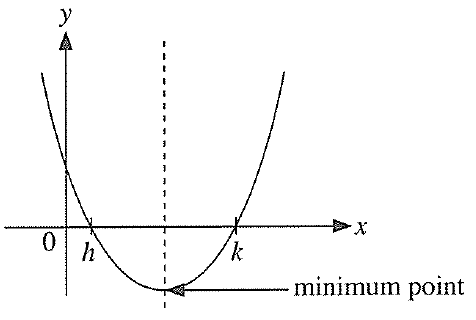
\includegraphics[width=0.35\textwidth]{05.png}

The graph intersects the $x$-axis at $(h,0)$ and $(k,0)$. 

The line of symmetry is $x = \frac{h+k}{2}$.

The minimum point also occurs at $x = \frac{h+k}{2}$. To find the $y$-coordinate of the minimum point, substitute $x = \frac{h+k}{2}$ into the expression $y=ax^2+bx+c$.

\item  Suppose that a quadratic function $y=ax^2+bx+c$ ($a \neq 0$) can be factorized into $a(x-h)(x-k)$.

Consider the case where $a < 0$. The graph is concave downwards (sad face) and there is a maximum point.

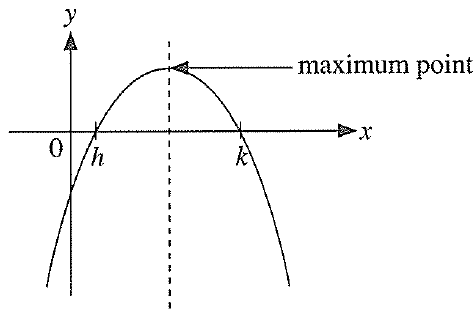
\includegraphics[width=0.35\textwidth]{06.png}

The graph intersects the $x$-axis at $(h,0)$ and $(k,0)$. 

The line of symmetry is $x = \frac{h+k}{2}$.

The maximum point also occurs at $x = \frac{h+k}{2}$. To find the $y$-coordinate of the maximum point, substitute $x = \frac{h+k}{2}$ into the expression $y=ax^2+bx+c$.

\item Suppose we complete the square quadratic function $y=ax^2+bx+c$ ($a \neq 0$) to obtain $y = a(x-p)^2 + q$.

If $a > 0$, then the graph is smiley face, and has a minimum point at $(p,q)$. The minimum value of $y$ is $q$. 

The equation $ax^2+bx+c = h$ has two solutions if $h > q$, one solution if $h=q$, and no solutions if $h < q$.

The line of symmetry $x=p$.

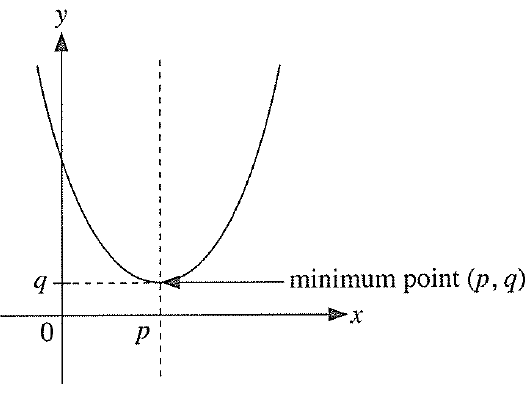
\includegraphics[width=0.35\textwidth]{07.png}

\item Suppose we complete the square quadratic function $y=ax^2+bx+c$ ($a \neq 0$) to obtain $y = a(x-p)^2 + q$.

If $a < 0$, then the graph is sad face, and has a maximum point at $(p,q)$. The maximum value of $y$ is $q$. 

The equation $ax^2+bx+c = h$ has two solutions if $h < q$, one solution if $h=q$, and no solutions if $h > q$.

The line of symmetry $x=p$. 

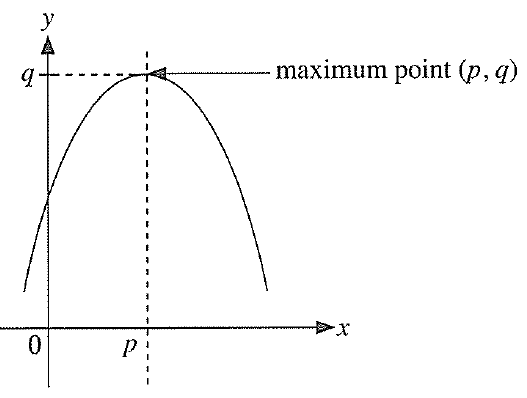
\includegraphics[width=0.35\textwidth]{08.png}

\section*{Coordinate Geometry}

\begin{itemize}

\item The length of a line segment with end points $A\left(x_1, y_1\right)$ and $B\left(x_2, y_2\right)$ is given by

$\sqrt{\left(x_1-x_2\right)^2+\left(y_1-y_2\right)^2}$ 

or equivalently

$\sqrt{\left(x_2-x_1\right)^2+\left(y_2-y_1\right)^2}$ 

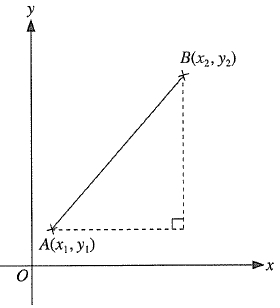
\includegraphics[width=0.3\textwidth]{15.png}

\item The gradient of a line passing through $A\left(x_1, y_1\right)$ and $B\left(x_2, y_2\right)$ is given by

$$\frac{y_2-y_1}{x_2-x_1}$$

or equivalently

$$\frac{y_1-y_2}{x_1-x_2}.$$

\item Collinear Points:

If gradient of $A B=$ gradient of $B C=$ gradient of $A C$, we say that $A,B,C$ are collinear. This means that $A,B,C$ lie on the same straight line (not necessarily in the order $A-B-C$; it could also be in any order such as $B-C-A$.)

Note: For collinear points, we only need to check the equality of one pair of gradients, for example, gradient of $A B=$ gradient of $B C$. Then automatically,  gradient of $A B=$ gradient of $A C$ and gradient of $A C=$ gradient of $B C$ as well.

When checking that gradient of $A B=$ gradient of $B C$, there must be a common point (in this case, $B$) in order to conclude that the points are collinear.

If gradient of $A B=$ gradient of $C D$ (ie, no common points), then we cannot conclude any of the points are collinear.

\item A horizontal line is parallel to the $x$-axis.
If all the points on the line has $y$-coordinate equal to $b$, then the equation of the line is
$$
y=b \text {. }
$$

A vertical line is parallel to the $y$-axis.
If all the points on the line has $x$-coordinate equal to $a$, then the equation of the line is
$$
x=a \text {. }
$$

If a line has a gradient $m$ and $y$-intercept $c$, then its equation is
$$
y=m x+c .
$$

The equation $y=m x+c$ is known as the gradient-intercept form.

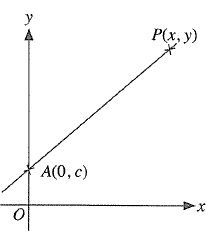
\includegraphics[width=0.2\textwidth]{16.png}


\end{itemize} 

\section*{Graphs and Functions}

Below is a summary of the graphs of the form $y=a x^n$, where $n=-2,-1,0,1,2$ and 3.

In the below sketches, we have assumed $a > 0$.

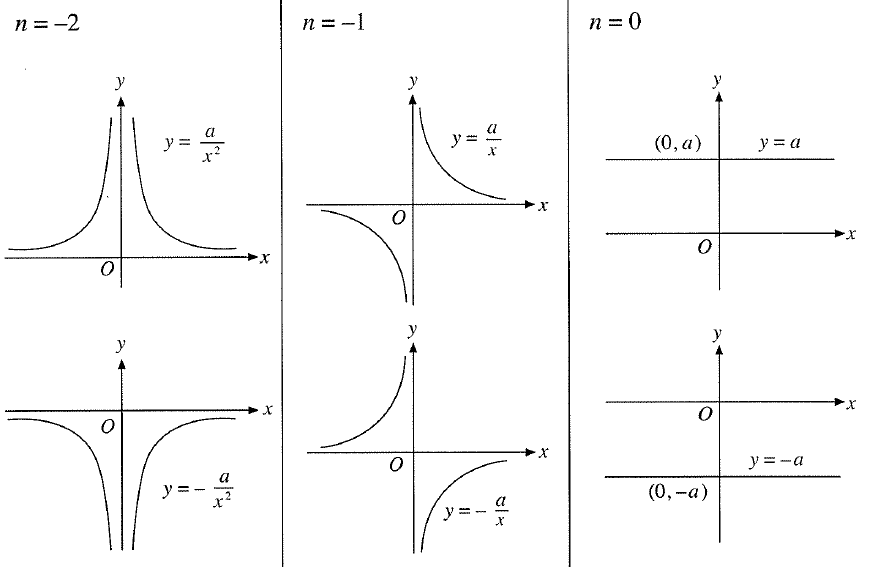
\includegraphics[width=0.48\textwidth]{09.png}

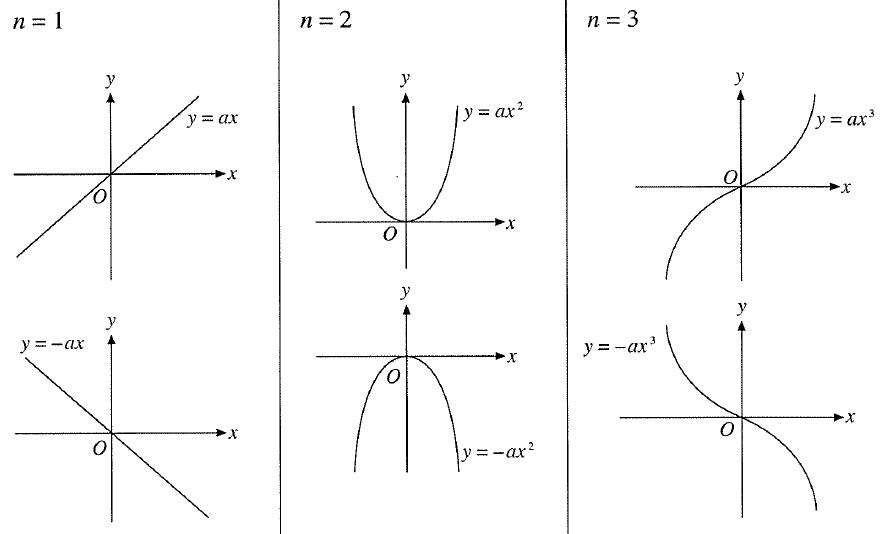
\includegraphics[width=0.48\textwidth]{10.png}

\bigskip 

\noindent 
These are graphs of the form $y = ka^x$.

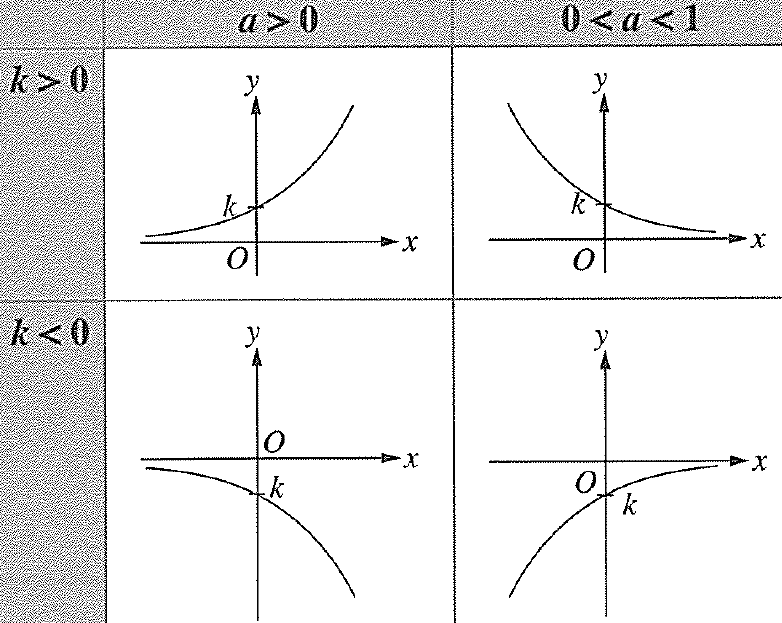
\includegraphics[width=0.48\textwidth]{11.png}

\bigskip 

\noindent 
Tangent to graphs:

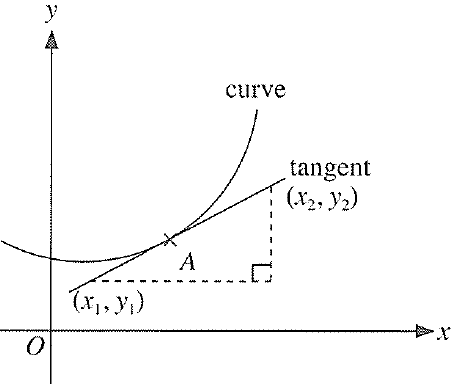
\includegraphics[width=0.4\textwidth]{12.png}

\bigskip 

\noindent 
A straight line which touches a curve at a single point $A$ is called a tangent to the curve at the point $A$.

\bigskip 

\noindent 
The gradient of the curve at the point $A$ is equal to the gradient of the tangent to the curve at $A$. In general, the gradient of the curve at any point is equal to the gradient of the tangent to the curve at that point.

\bigskip 

\noindent 
Distance-Time Graphs:

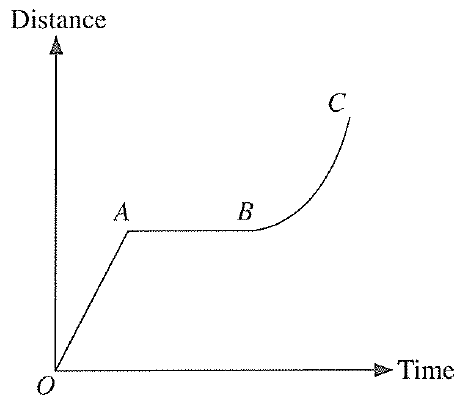
\includegraphics[width=0.3\textwidth]{13.png}

\noindent 
The gradient of a distance-time graph gives the speed of the object.

\noindent 
$O A$ is a straight line, i.e. speed of object $=$ gradient of $O A$.

\noindent 
$A B$ is a horizontal line, i.e. speed of object $=$ zero.

\noindent 
$B C$ is a curve, i.e. instantaneous speed of object $=$ gradient of the tangent to the curve at a point.

\bigskip

\noindent
Various types of distance-time graphs:

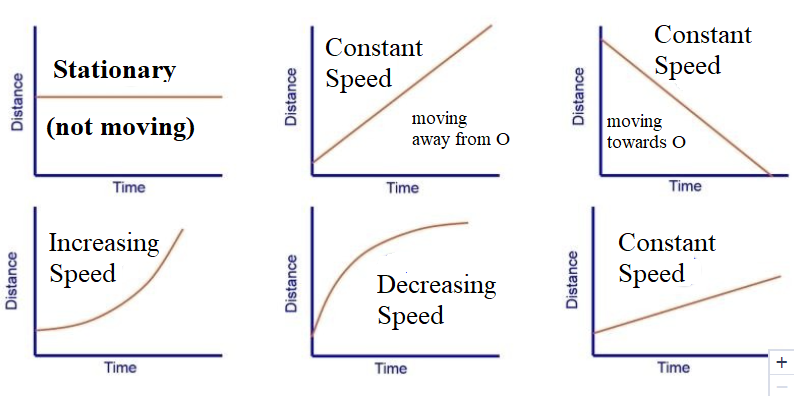
\includegraphics[width=0.5\textwidth]{17.png}

\bigskip 

\bigskip 

\noindent 
Speed-Time Graphs:

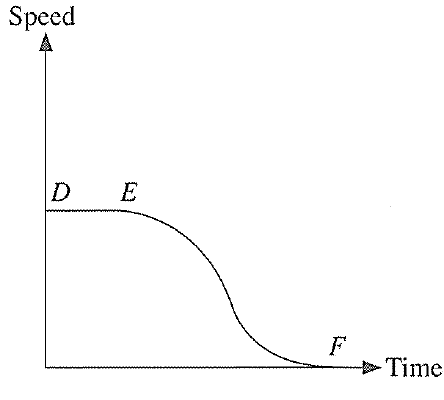
\includegraphics[width=0.3\textwidth]{14.png}

\noindent 
The gradient of a speed-time graph gives the acceleration of the object.

\noindent 
The area under a speed-time graph gives the distance travelled by the object.

\noindent 
$D E$ is a horizontal line, i.e. acceleration of object $=$ zero.

\noindent 
$E F$ is a curve, i.e. instantaneous acceleration of object $=$ gradient of tangent to the curve at a point.

\noindent 
Total distance travelled $=$ area under graph from $D$ to $F$

\bigskip

\noindent
Various types of speed-time graphs:

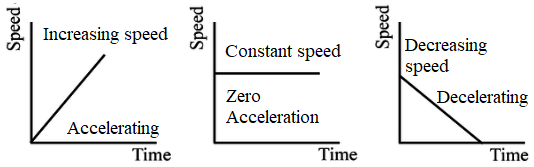
\includegraphics[width=0.5\textwidth]{18.png}

\newpage 

\section*{Angles, Triangles, Polygons}

\noindent
Types of angles:

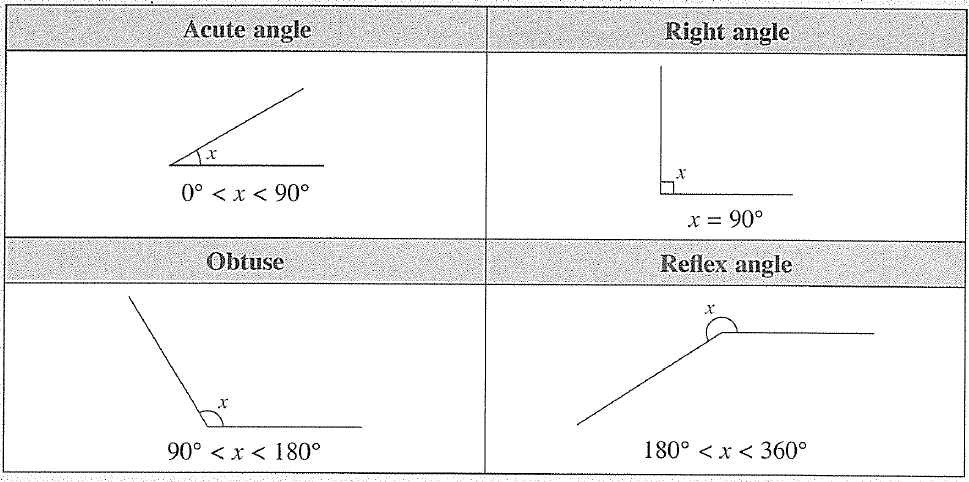
\includegraphics[width=0.5\textwidth]{19.png}

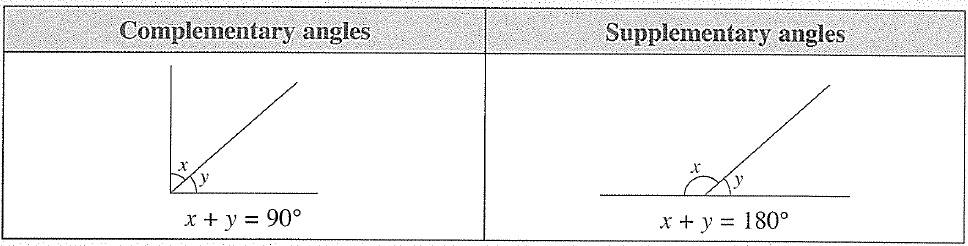
\includegraphics[width=0.5\textwidth]{22.png}

\noindent
Geometric properties of parallel lines and angles:

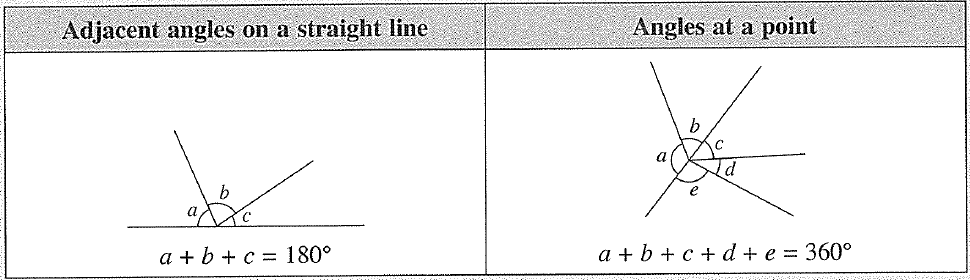
\includegraphics[width=0.5\textwidth]{20.png}

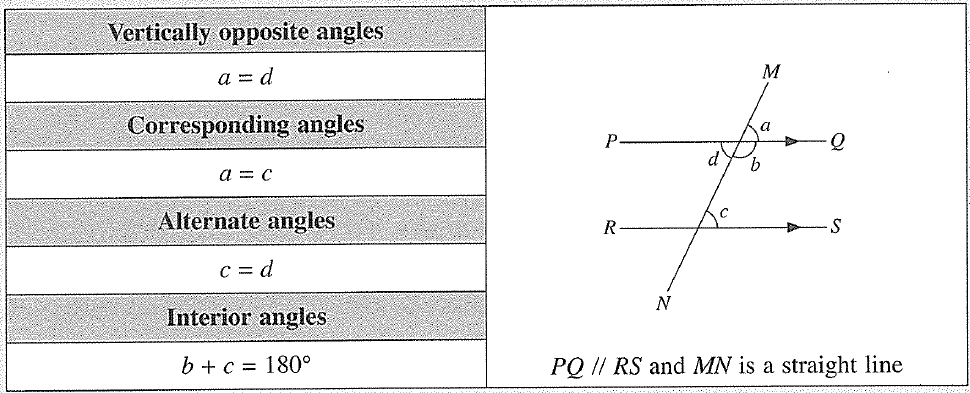
\includegraphics[width=0.5\textwidth]{21.png}

Types of triangles:

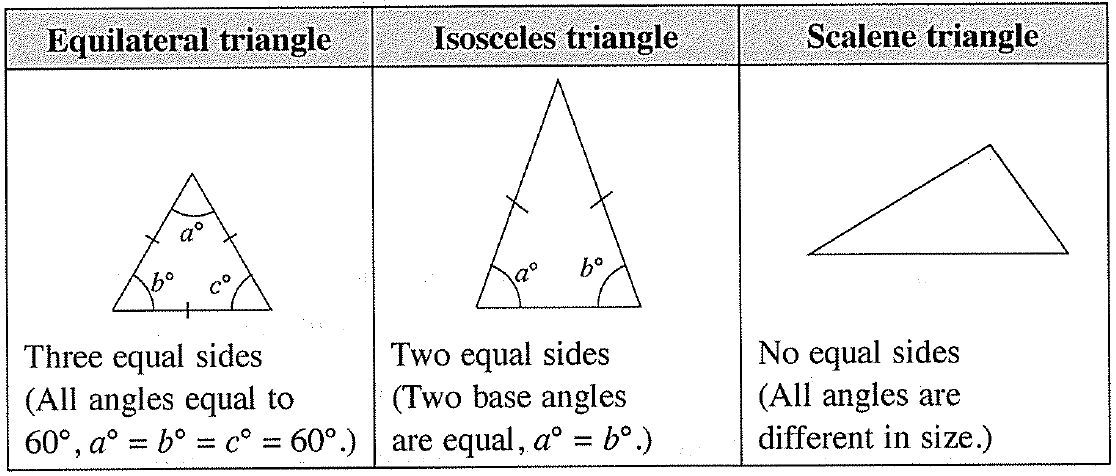
\includegraphics[width=0.5\textwidth]{23.png}

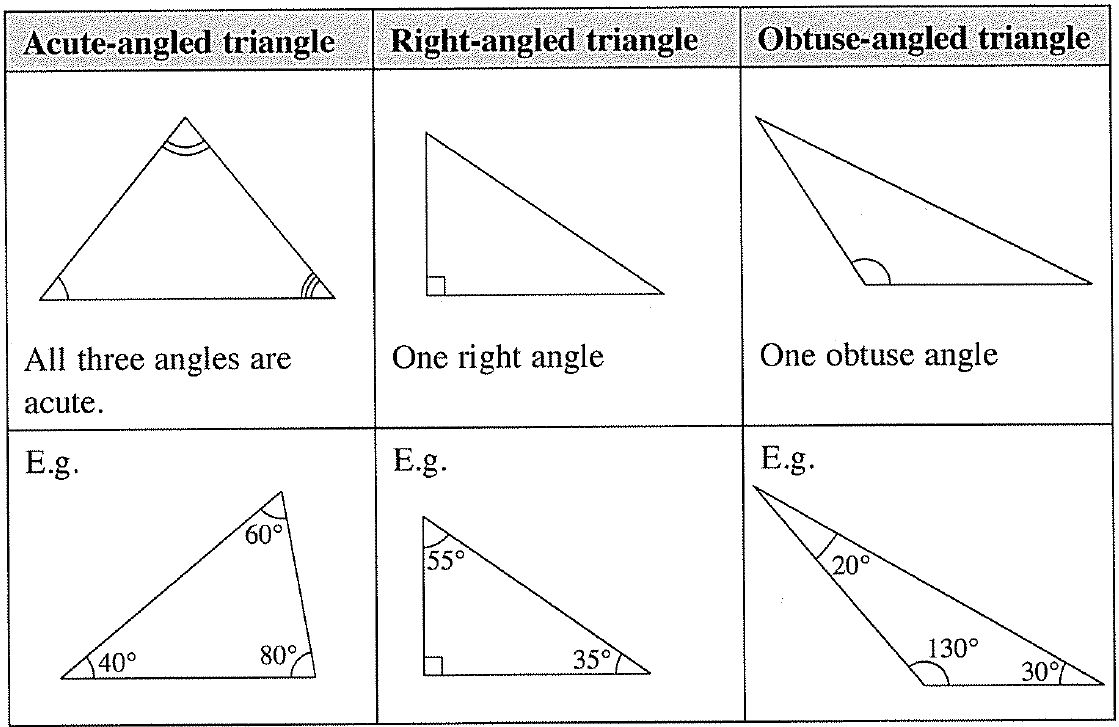
\includegraphics[width=0.5\textwidth]{24.png}

\noindent
Types of quadrilaterals:

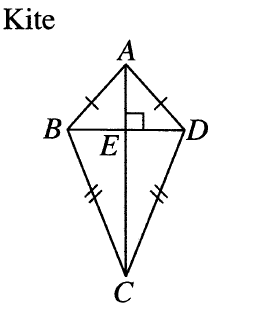
\includegraphics[width=0.175\textwidth]{32.png} \\
1. $AB=AD$ and $CB=CD$ \\
2. Both $\triangle A B D$ and $\triangle B C D$ are isosceles, with $\angle A B D=\angle A D B$ and $\angle B D C=\angle D B C$ \\
3. Diagonals $A C$ and $B D$ intersect each other at right angles at $E$ \\
4. The longer diagonal $A C$ bisects the shorter diagonal $B D$ 

\bigskip

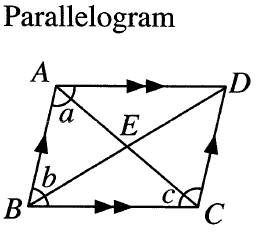
\includegraphics[width=0.175\textwidth]{30.png} \\
1. Opposite sides are parallel and are of equal length. \\
2. $\angle a+\angle b=180^{\circ}$ (int. $\angle \mathrm{s}$ ) \\
3. Opposite angles are equal, i.e. $\angle a=\angle c$ \\
(opp. $\angle \mathrm{s}$ of parallelogram) \\
4. Diagonals $A C$ and $B D$ bisect each other at $E$, i.e. 
$A E=E C$ and $B E=E D$, in other words, $E$ is the mid-point of $AC$ and $BD$.

\bigskip

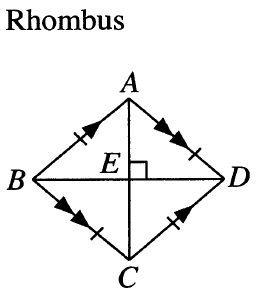
\includegraphics[width=0.175\textwidth]{33.png} \\
1. Opposite sides are parallel. \\
2. All four sides are equal in length \\
3. $\angle A B C+\angle B C D = 180^{\circ}$ $\text { (int. } \angle \mathrm{s} \text { ) }$ \\
4. Opposite angles are equal, i.e. $\angle A B C=\angle A D C  \text { and } \angle B A D=\angle B C D$ \\
5. The diagonals bisect the interior angles, so that $\angle A B D = \angle C B D$ and $\angle A D B = \angle C D B$ \\
6. Both $\triangle A B D$ and $\triangle B C D$ are isosceles, with $\angle A B D=\angle A D B$ and $\angle C B D=\angle C D B$ \\
7. Diagonals $A C$ and $B D$ bisect each other at right angles, in other words, they are perpendicular bisectors of each other

\bigskip

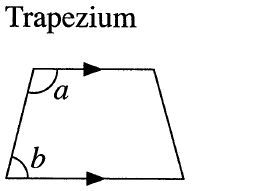
\includegraphics[width=0.175\textwidth]{31.png} \\
1. One pair of parallel sides. \\
2. $\angle a+\angle b=180^{\circ}$	(int. $\angle \mathrm{s})$ \\
3. Note that the pair of opposite parallel sides may not be same length\\
4. Also, it may be that none of the interior angles are equal

\bigskip

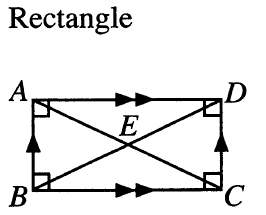
\includegraphics[width=0.175\textwidth]{34.png} \\
1. Same properties as parallelogram. \\
2. In addition, the diagonals $AC$ and $BD$ are of equal length (in a parallelogram, the diagonals may not be of equal length) \\
3. Each interior angle is $90^\circ$. \\
4. $\triangle AED$, $\triangle AEB$, $\triangle BEC$ and $\triangle CED$ are isosceles triangles.

\bigskip

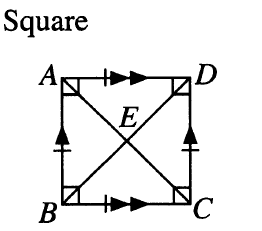
\includegraphics[width=0.175\textwidth]{35.png} \\
1. Same properties as rhombus. \\
2. In addition, the diagonals $AC$ and $BD$ are of equal length (in a rhombus, the diagonals may not be of equal length) \\
3. Each interior angle is $90^\circ$. \\
4. Each of the four triangles $\triangle AED$, $\triangle AEB$, $\triangle BEC$ and $\triangle CED$ are isosceles right-angled triangles whose base angles are each $45^\circ$.

\bigskip

\noindent
Angle properties of polygons:

\bigskip

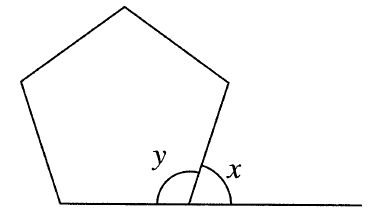
\includegraphics[width=0.25\textwidth]{40.png} \\
1. In a polygon, the sum of an interior angle and its corresponding exterior angle is $180^{\circ}$, i.e. $\angle x+\angle y=180^{\circ}$. \\
2. The sum of exterior angles of an $n$-sided polygon is $360^{\circ}$. \\
3. In the case of a $n$-sided regular polygon, each exterior angle, $\angle x=\frac{360^{\circ}}{n}$. \\
4. The sum of interior angles of an $n$-sided polygon is $(n-2) \times 180^{\circ}$. \\
5. In the case of a $n$-sided regular polygon, each interior angle, $\angle y=\frac{(n-2) \times 180^{\circ}}{n}$.

\begin{tabular}{|c|c|}
	\hline \begin{tabular}{c} 
		No. of sides \\
		$(\boldsymbol{n})$
	\end{tabular} & Name of Polygon \\
	\hline 3 & Triangle \\
	\hline 4 & Quadrilateral \\
	\hline 5 & Pentagon \\
	\hline 6 & Hexagon \\
	\hline 7 & Heptagon \\
	\hline 8 & Octagon \\
	\hline 9 & Nonagon \\
	\hline 10 & Decagon \\
	\hline
\end{tabular}

\end{enumerate}

\section*{Geometric Constructions}

\noindent
Constructing Perpendicular Bisector of a given line segment $XY$:

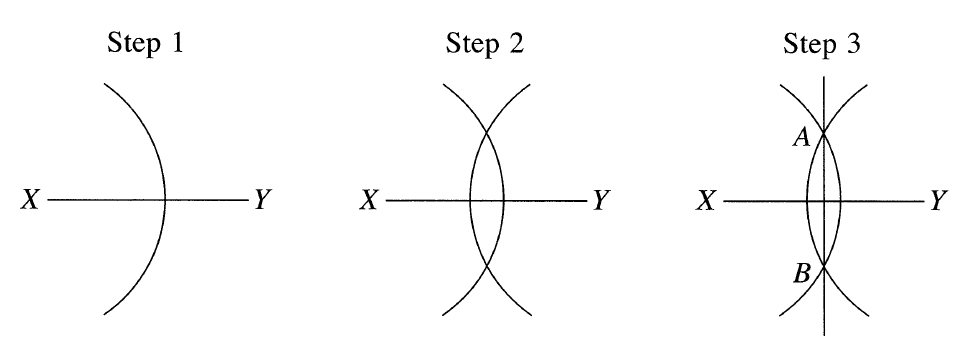
\includegraphics[width=0.5\textwidth]{53.png}

\noindent
1. Put your compass on point $X$ and set it to be more than half the length of line segment $X Y$.
Draw an arc.

\noindent
2. Without adjusting the length of your compass, put it on point $Y$. Draw another arc of the same radius to cut the first arc above and below the line segment $X Y$.

\noindent
3. Label the points of intersection of the two arcs as $A$ and $B$ respectively. Draw a line passing through $A$ and $B$. The line $A B$ is the perpendicular bisector of the line segment $X Y$.

\noindent
Any point $M$ on the perpendicular bisector of the line segment $XY$ is equidistant from the points $X$ and $Y$, i.e. $X M=Y M$.

\bigskip 

\noindent
Constructing Angle Bisector:

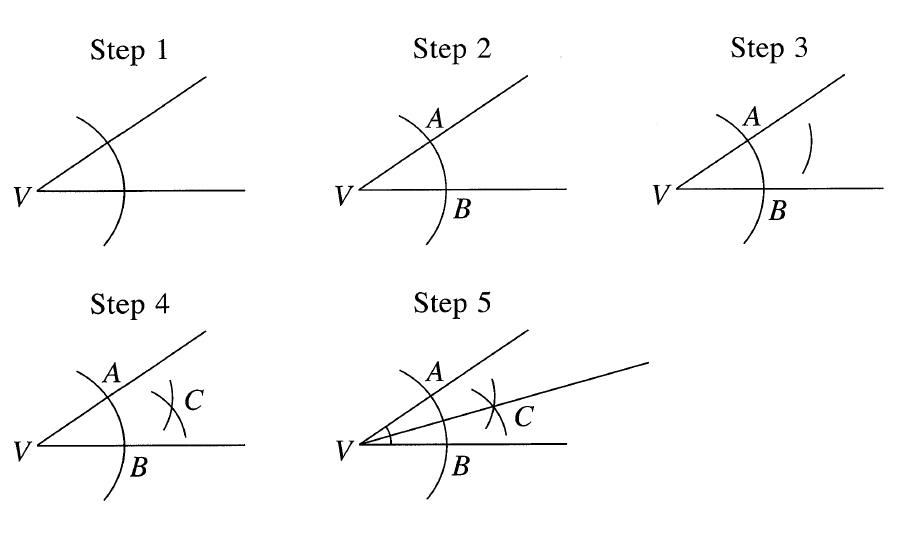
\includegraphics[width=0.5\textwidth]{55.png}

\noindent 
1. Place your compass on point $V$ and draw an arc that crosses both sides of the angle. Label the two intersection points as $A$ and $B$.

\noindent 
2. Place your compass on point $A$ and draw an arc of any suitable radius between the two sides of the angle.

\noindent 
3. Without adjusting the length of your compass, place it on point $B$ and draw another arc of the same radius as the arc drawn in Step 2. Label the point where the two arcs meet as $C$.

\noindent 
4. Draw a straight line through $V$ and $C$. The line $V C$ is the angle bisector of $\angle V$ where $\angle A V C=\angle B V C$.

\noindent
Any point $P$ on the angle bisector of $\angle A V B$ is equidistant from the two lines $VA$ and $VB$.



\section*{Radian Measure, Perimeter and Area of Plane Figures, Arc Length and Area of Sector}

\noindent
Convert between radian and degrees:

\noindent
$\pi$ radian $=180^{\circ}$

\noindent
1 radian $=\frac{180^{\circ}}{\pi}$

\noindent 
$
1^{\circ}=\frac{\pi}{180^{\circ}} \text { radian }
$

\noindent
Examples: 

\noindent
2.1 radian $=2.1 \times \frac{180^{\circ}}{\pi} =120.3^{\circ} \text { (to } 1 \text { d.p.) } $

\noindent
$30^{\circ}=\frac{\pi}{180^{\circ}} \times 30^{\circ} =\frac{\pi}{6} \ \mathrm{rad}$

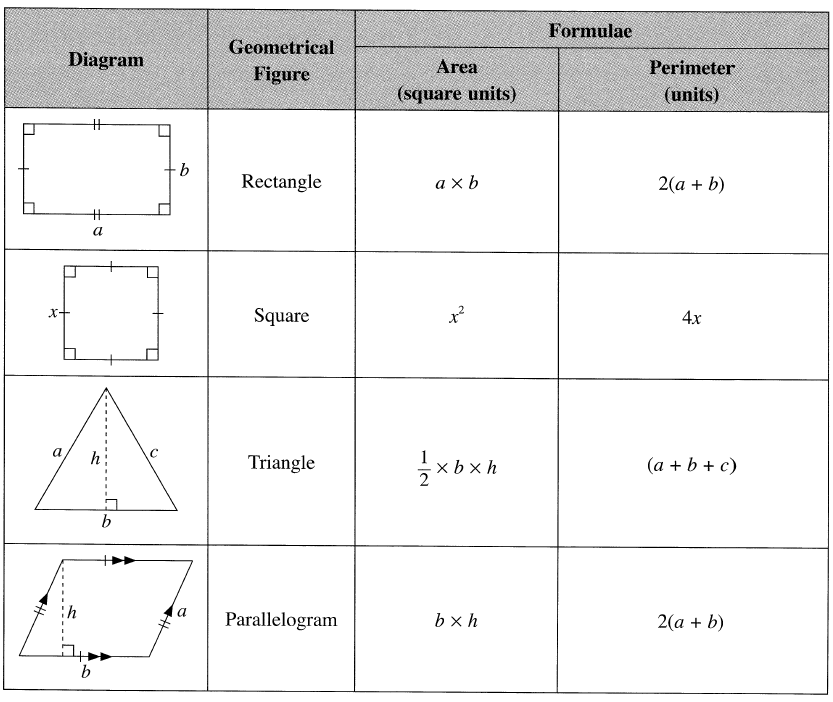
\includegraphics[width=0.45\textwidth]{80.png}

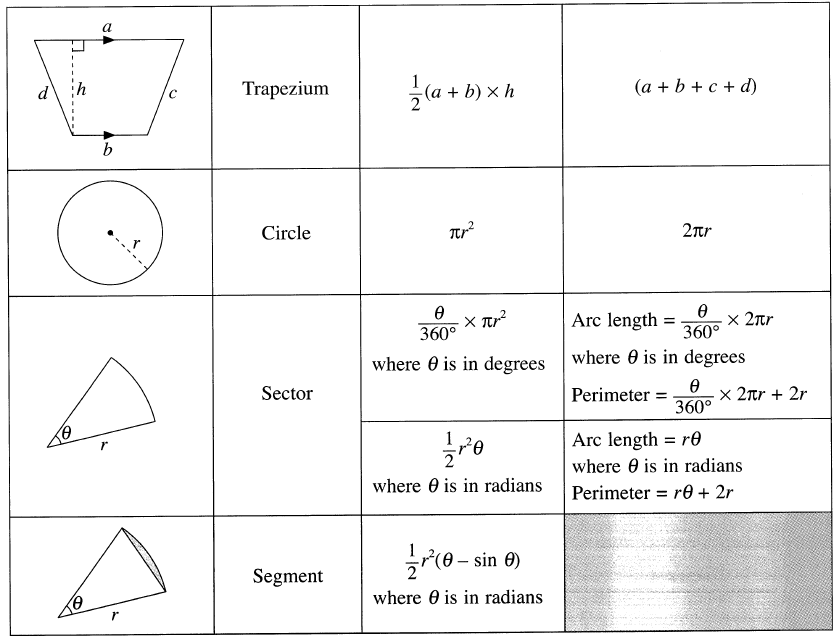
\includegraphics[width=0.5\textwidth]{81.png}

\section*{Surface Area and Volume of Solids}

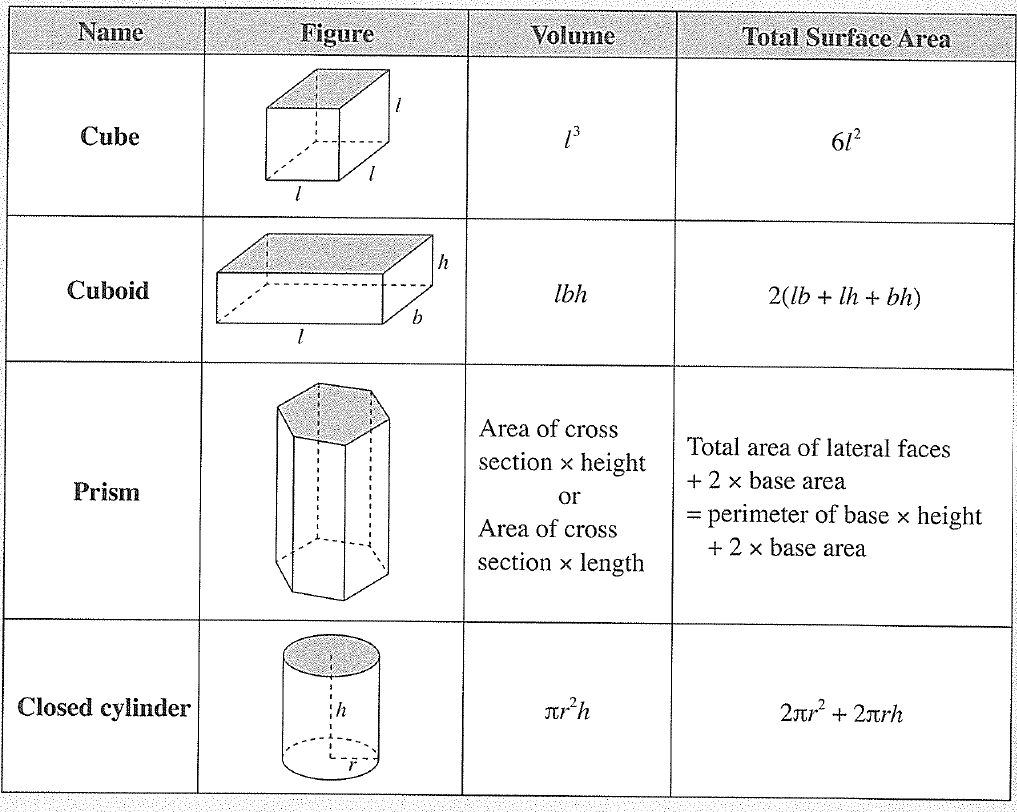
\includegraphics[width=0.5\textwidth]{82.png}

\end{document}